\documentclass{beamer}
\usetheme{metropolis}
\usepackage{graphicx}
\usepackage{subcaption}
\usepackage{hyperref}
\usepackage{tcolorbox}
\title{Algebra-Based Physics-1: Mechanics (PHYS135A-01): Summary}
\date{October 30th - November 3rd, 2017}
\author{Jordan Hanson}
\institute{Whittier College Department of Physics and Astronomy}

\begin{document}
\maketitle

\section{Course Summary}

\begin{frame}{Course Summary}
\begin{enumerate}
\item Unit 0 - Units, estimation, and vectors
\item Unit 1 - Kinematics
\item Unit 2 - Kinematics in More than One Dimension
\item Unit 3 - Midterm 1
\item Unit 4 - Newton's Laws of Motion
\item Unit 5 - Applications of Newton's Laws: friction, drag, elasticity
\item Midterm 2 - Midterm 2
\item Unit 6 - Uniform Circular Motion
\item Unit 7 - Work, Energy, and Energy Consumption
\item Unit 8 - Linear Momentum
\item Unit 9 - Rotational Dynamics
\end{enumerate}
\end{frame}

\section{It has been my pleasure.}

\begin{frame}{Thank you}
\begin{figure}
\centering
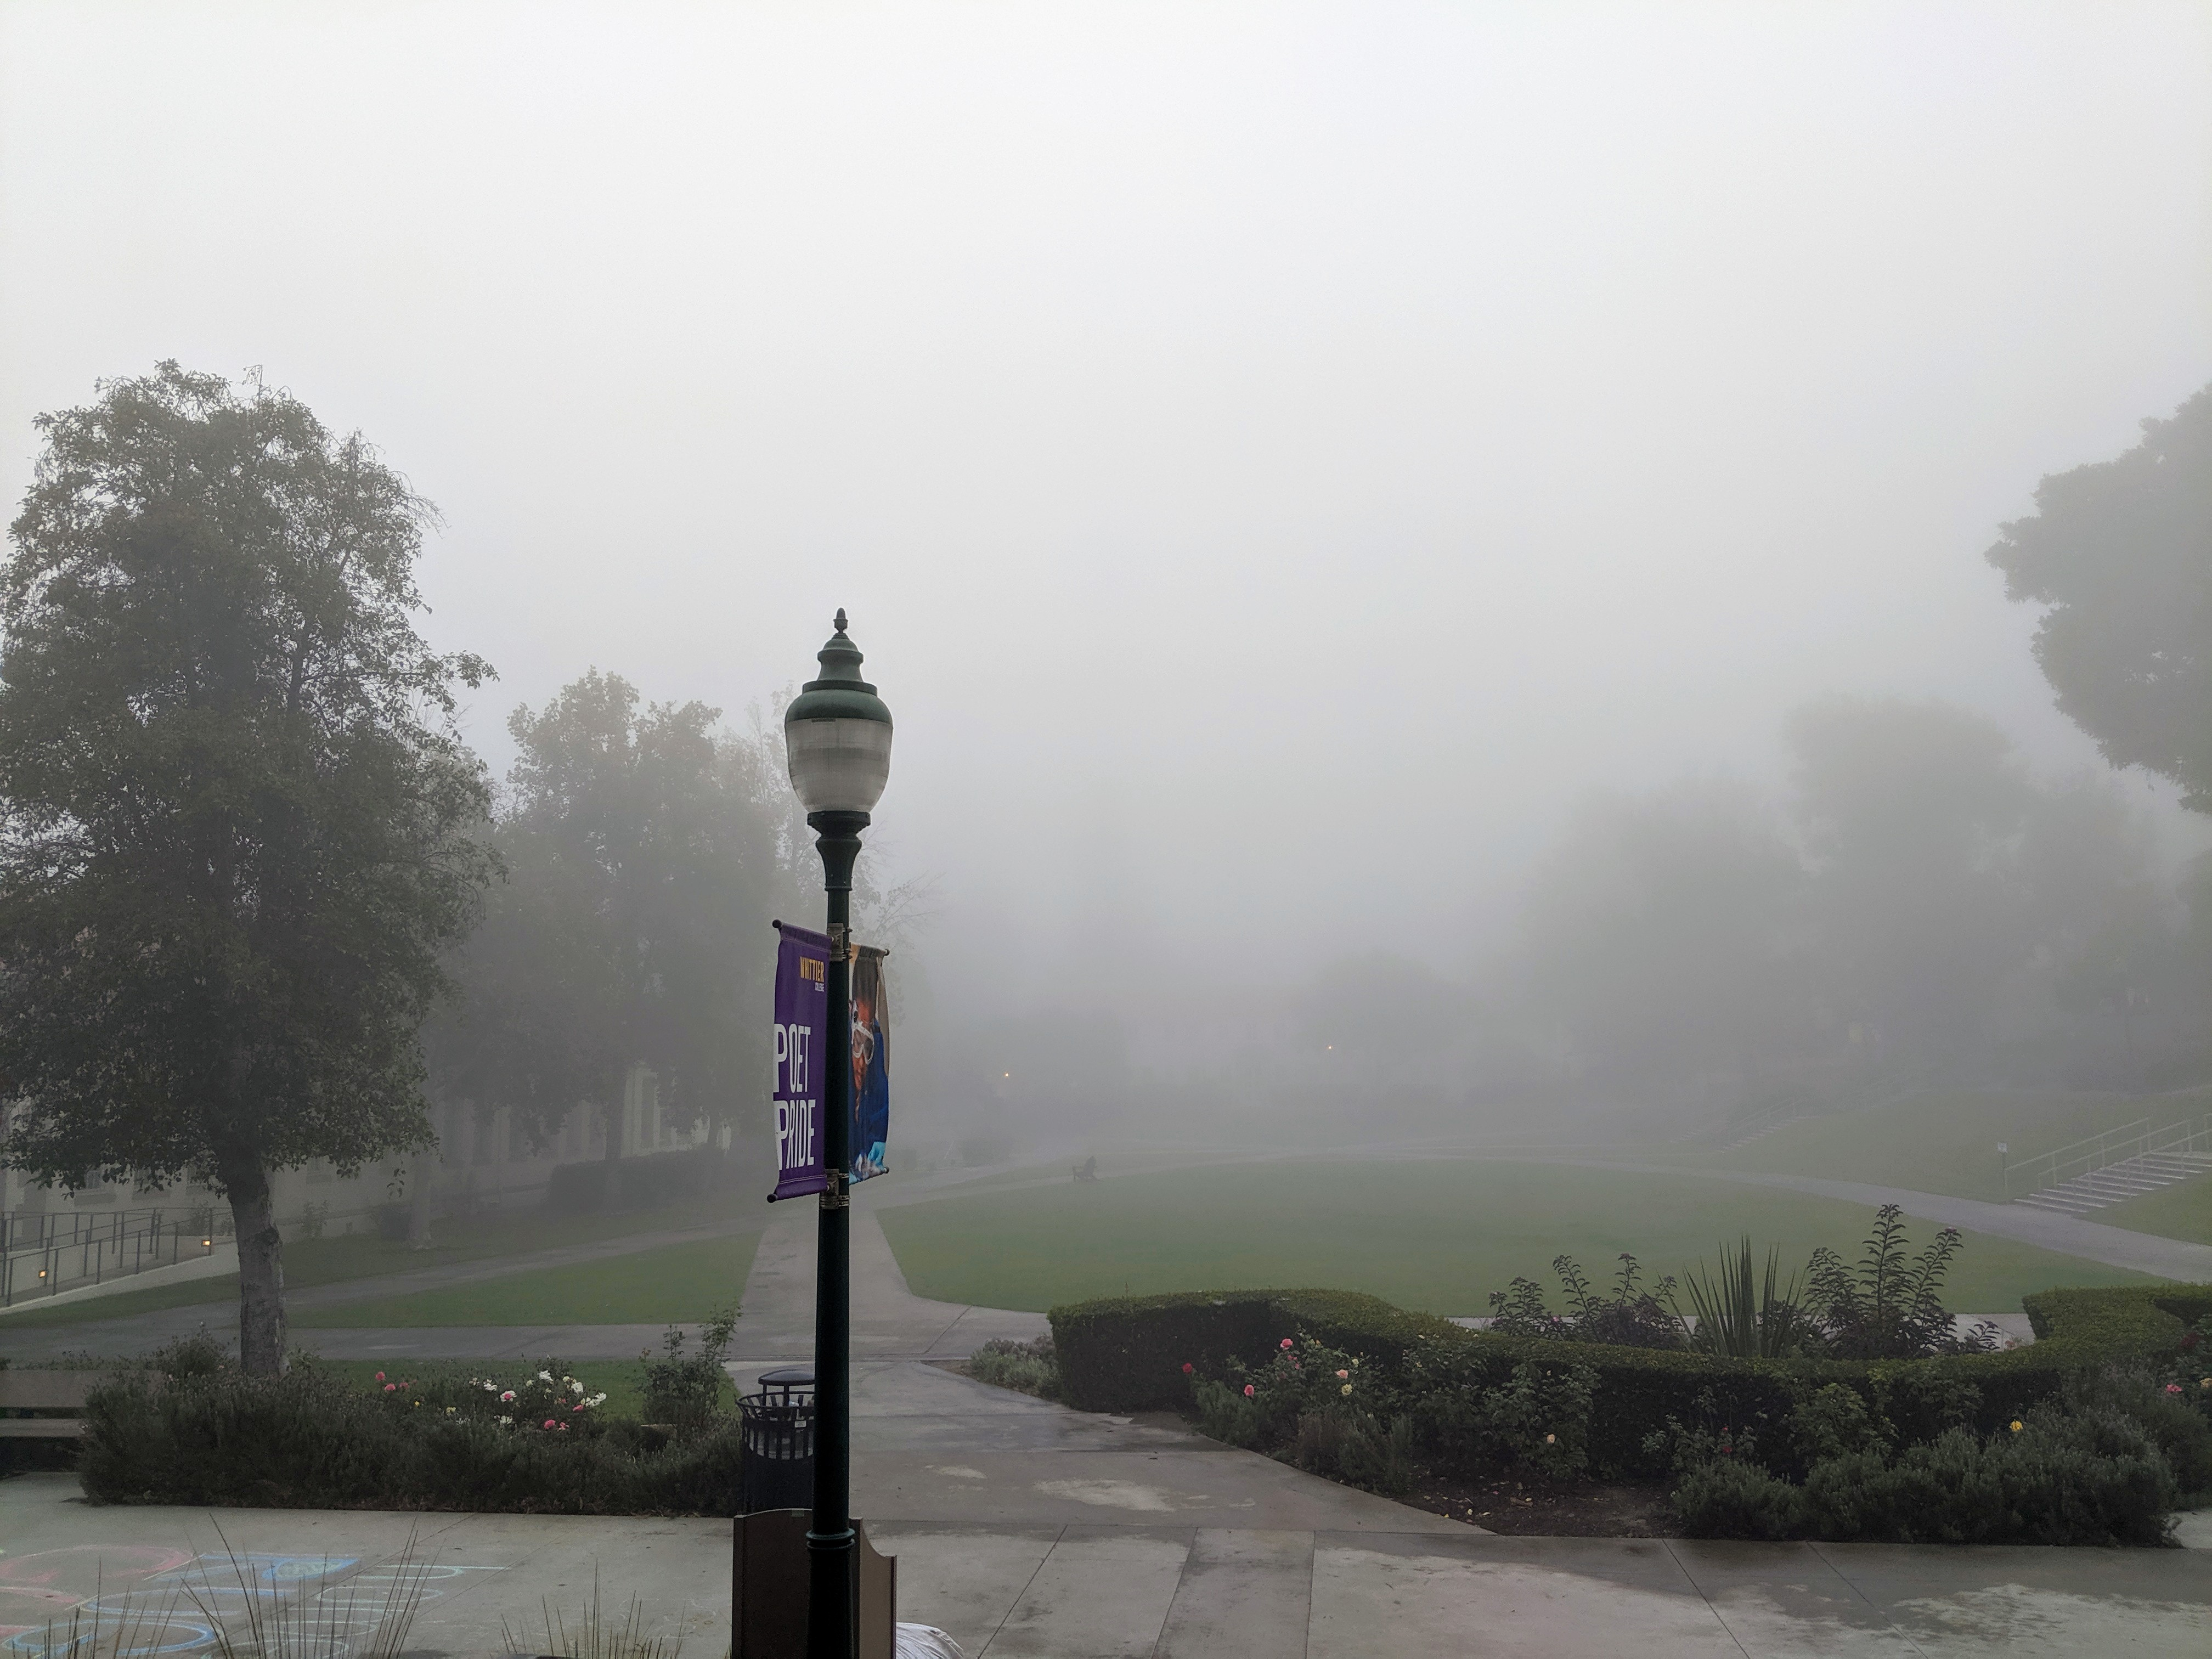
\includegraphics[width=0.75\textwidth]{IMG_20191112_074409.jpg}
\end{figure}
\end{frame}

\begin{frame}{Thank you}
\begin{figure}
\centering
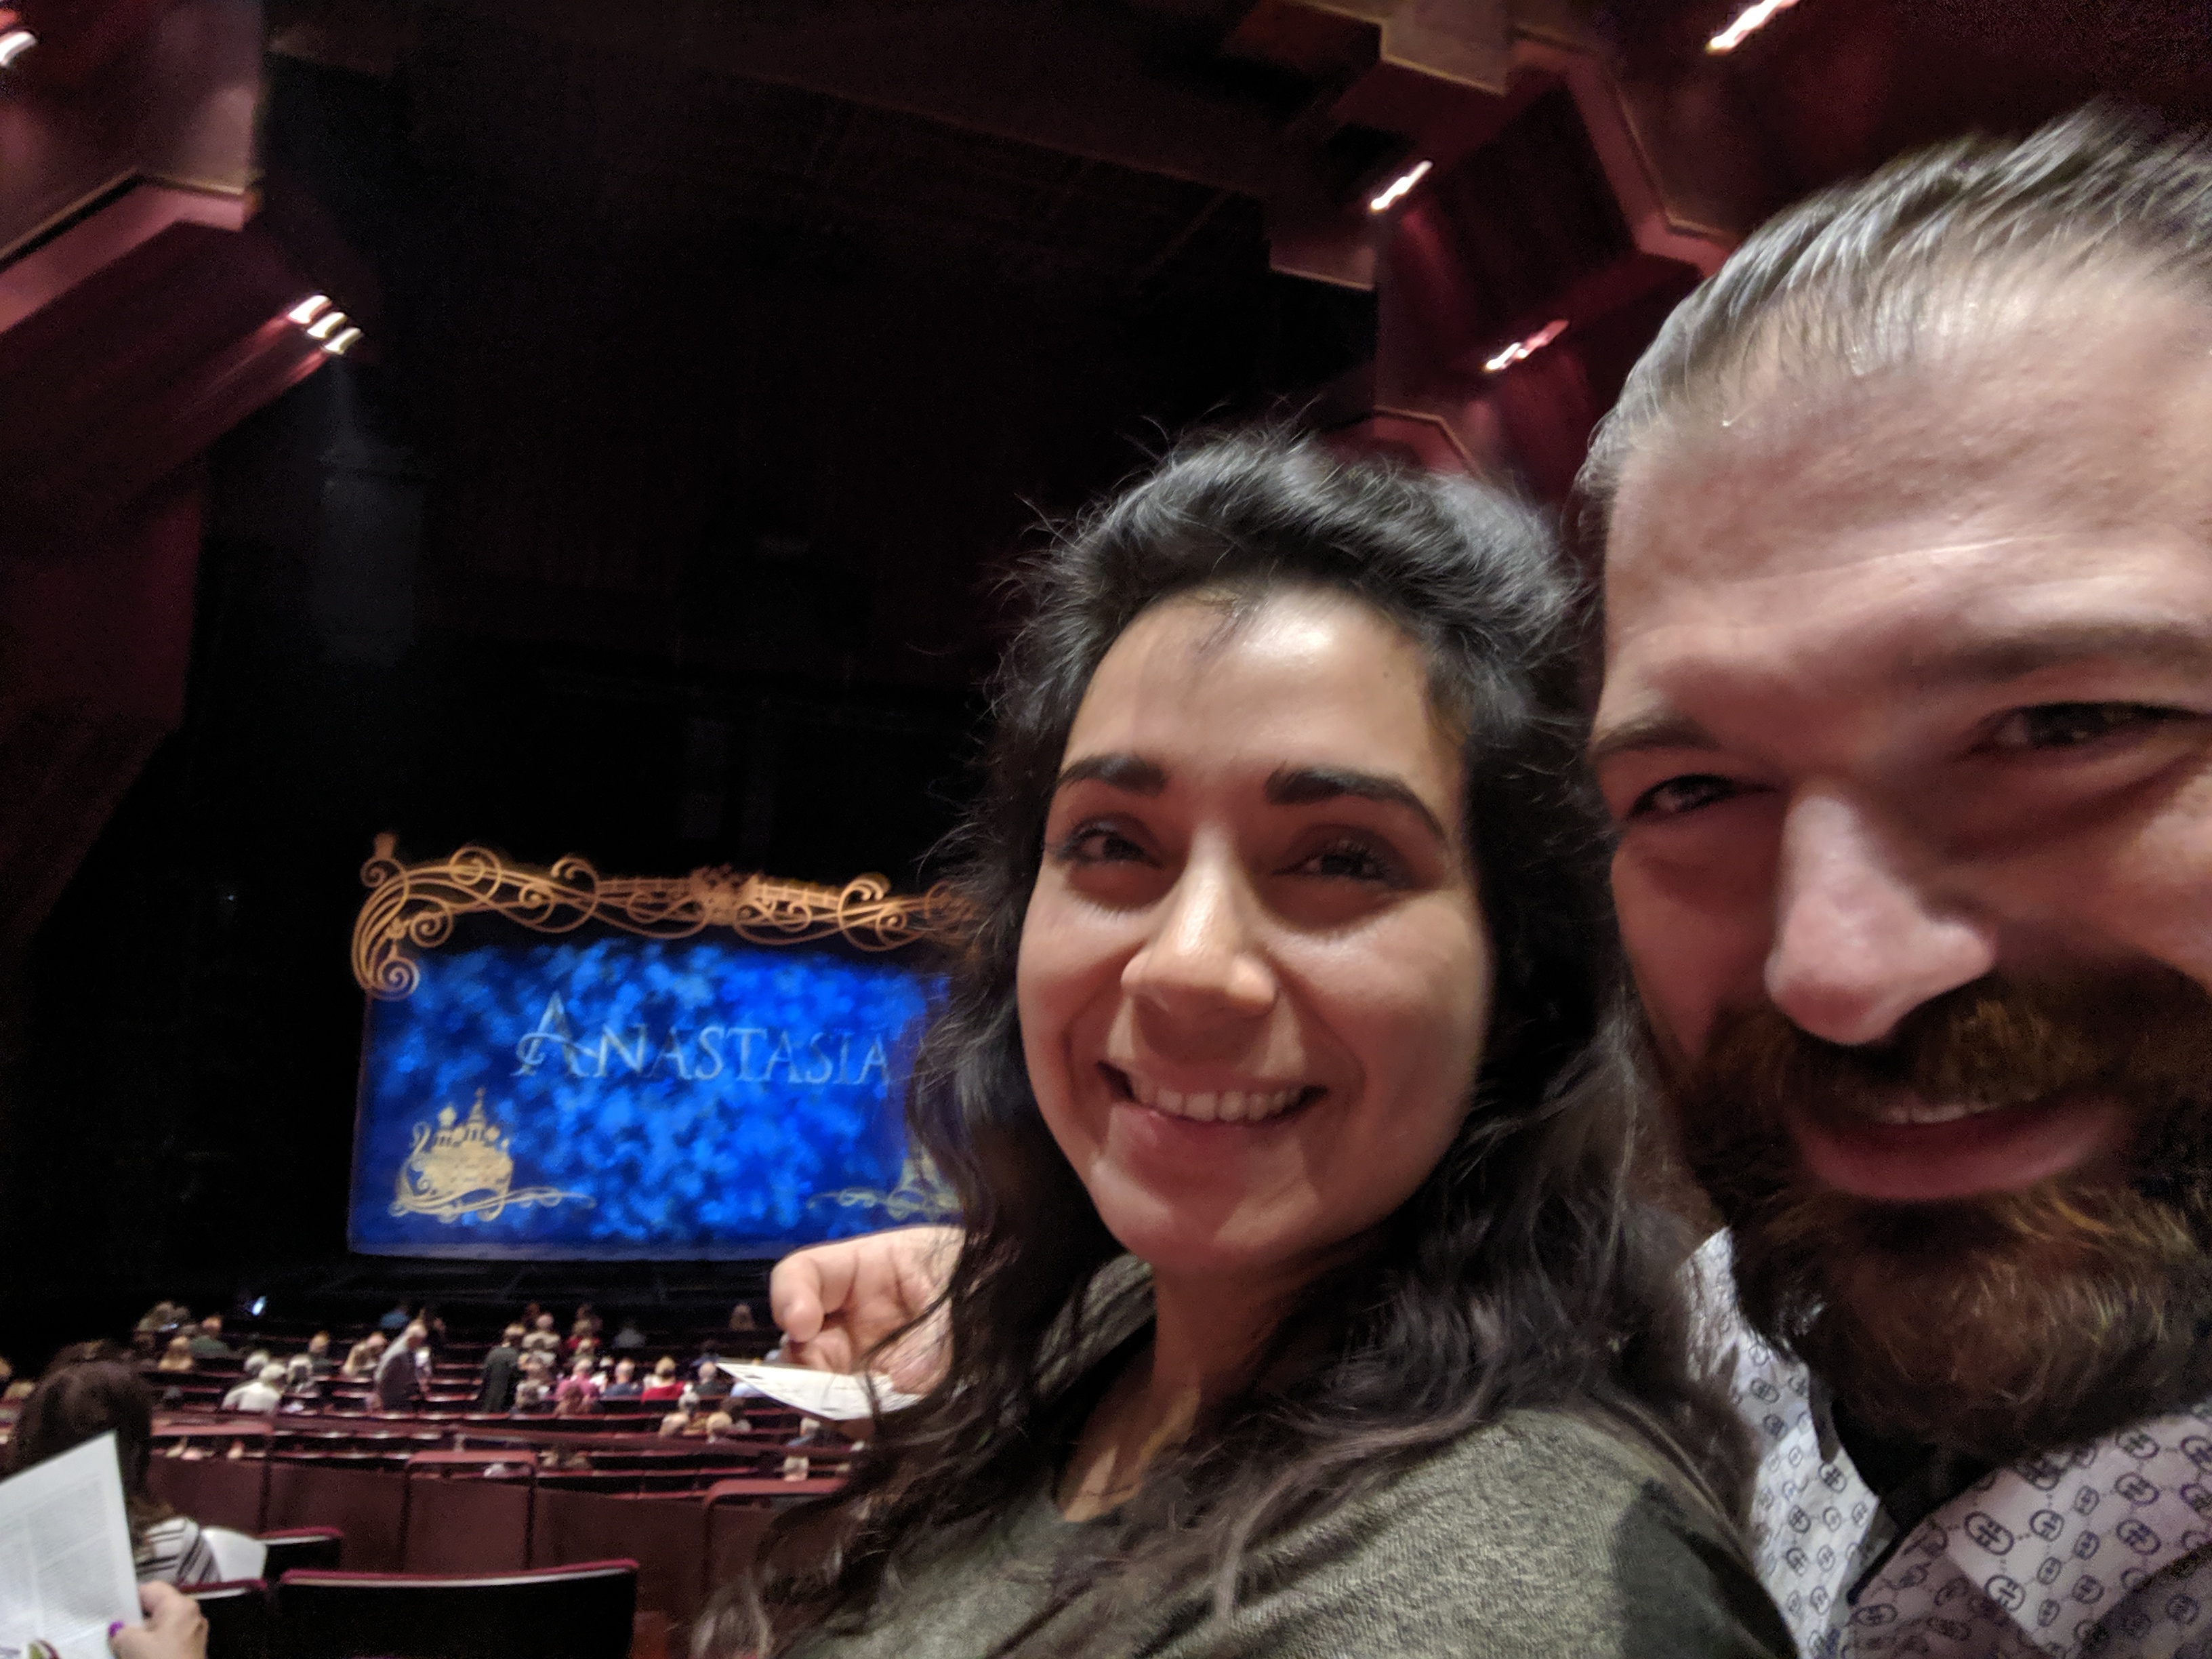
\includegraphics[width=0.75\textwidth]{IMG_20191109_191859.jpg}
\end{figure}
\end{frame}

\begin{frame}{Thank you}
\begin{figure}
\centering
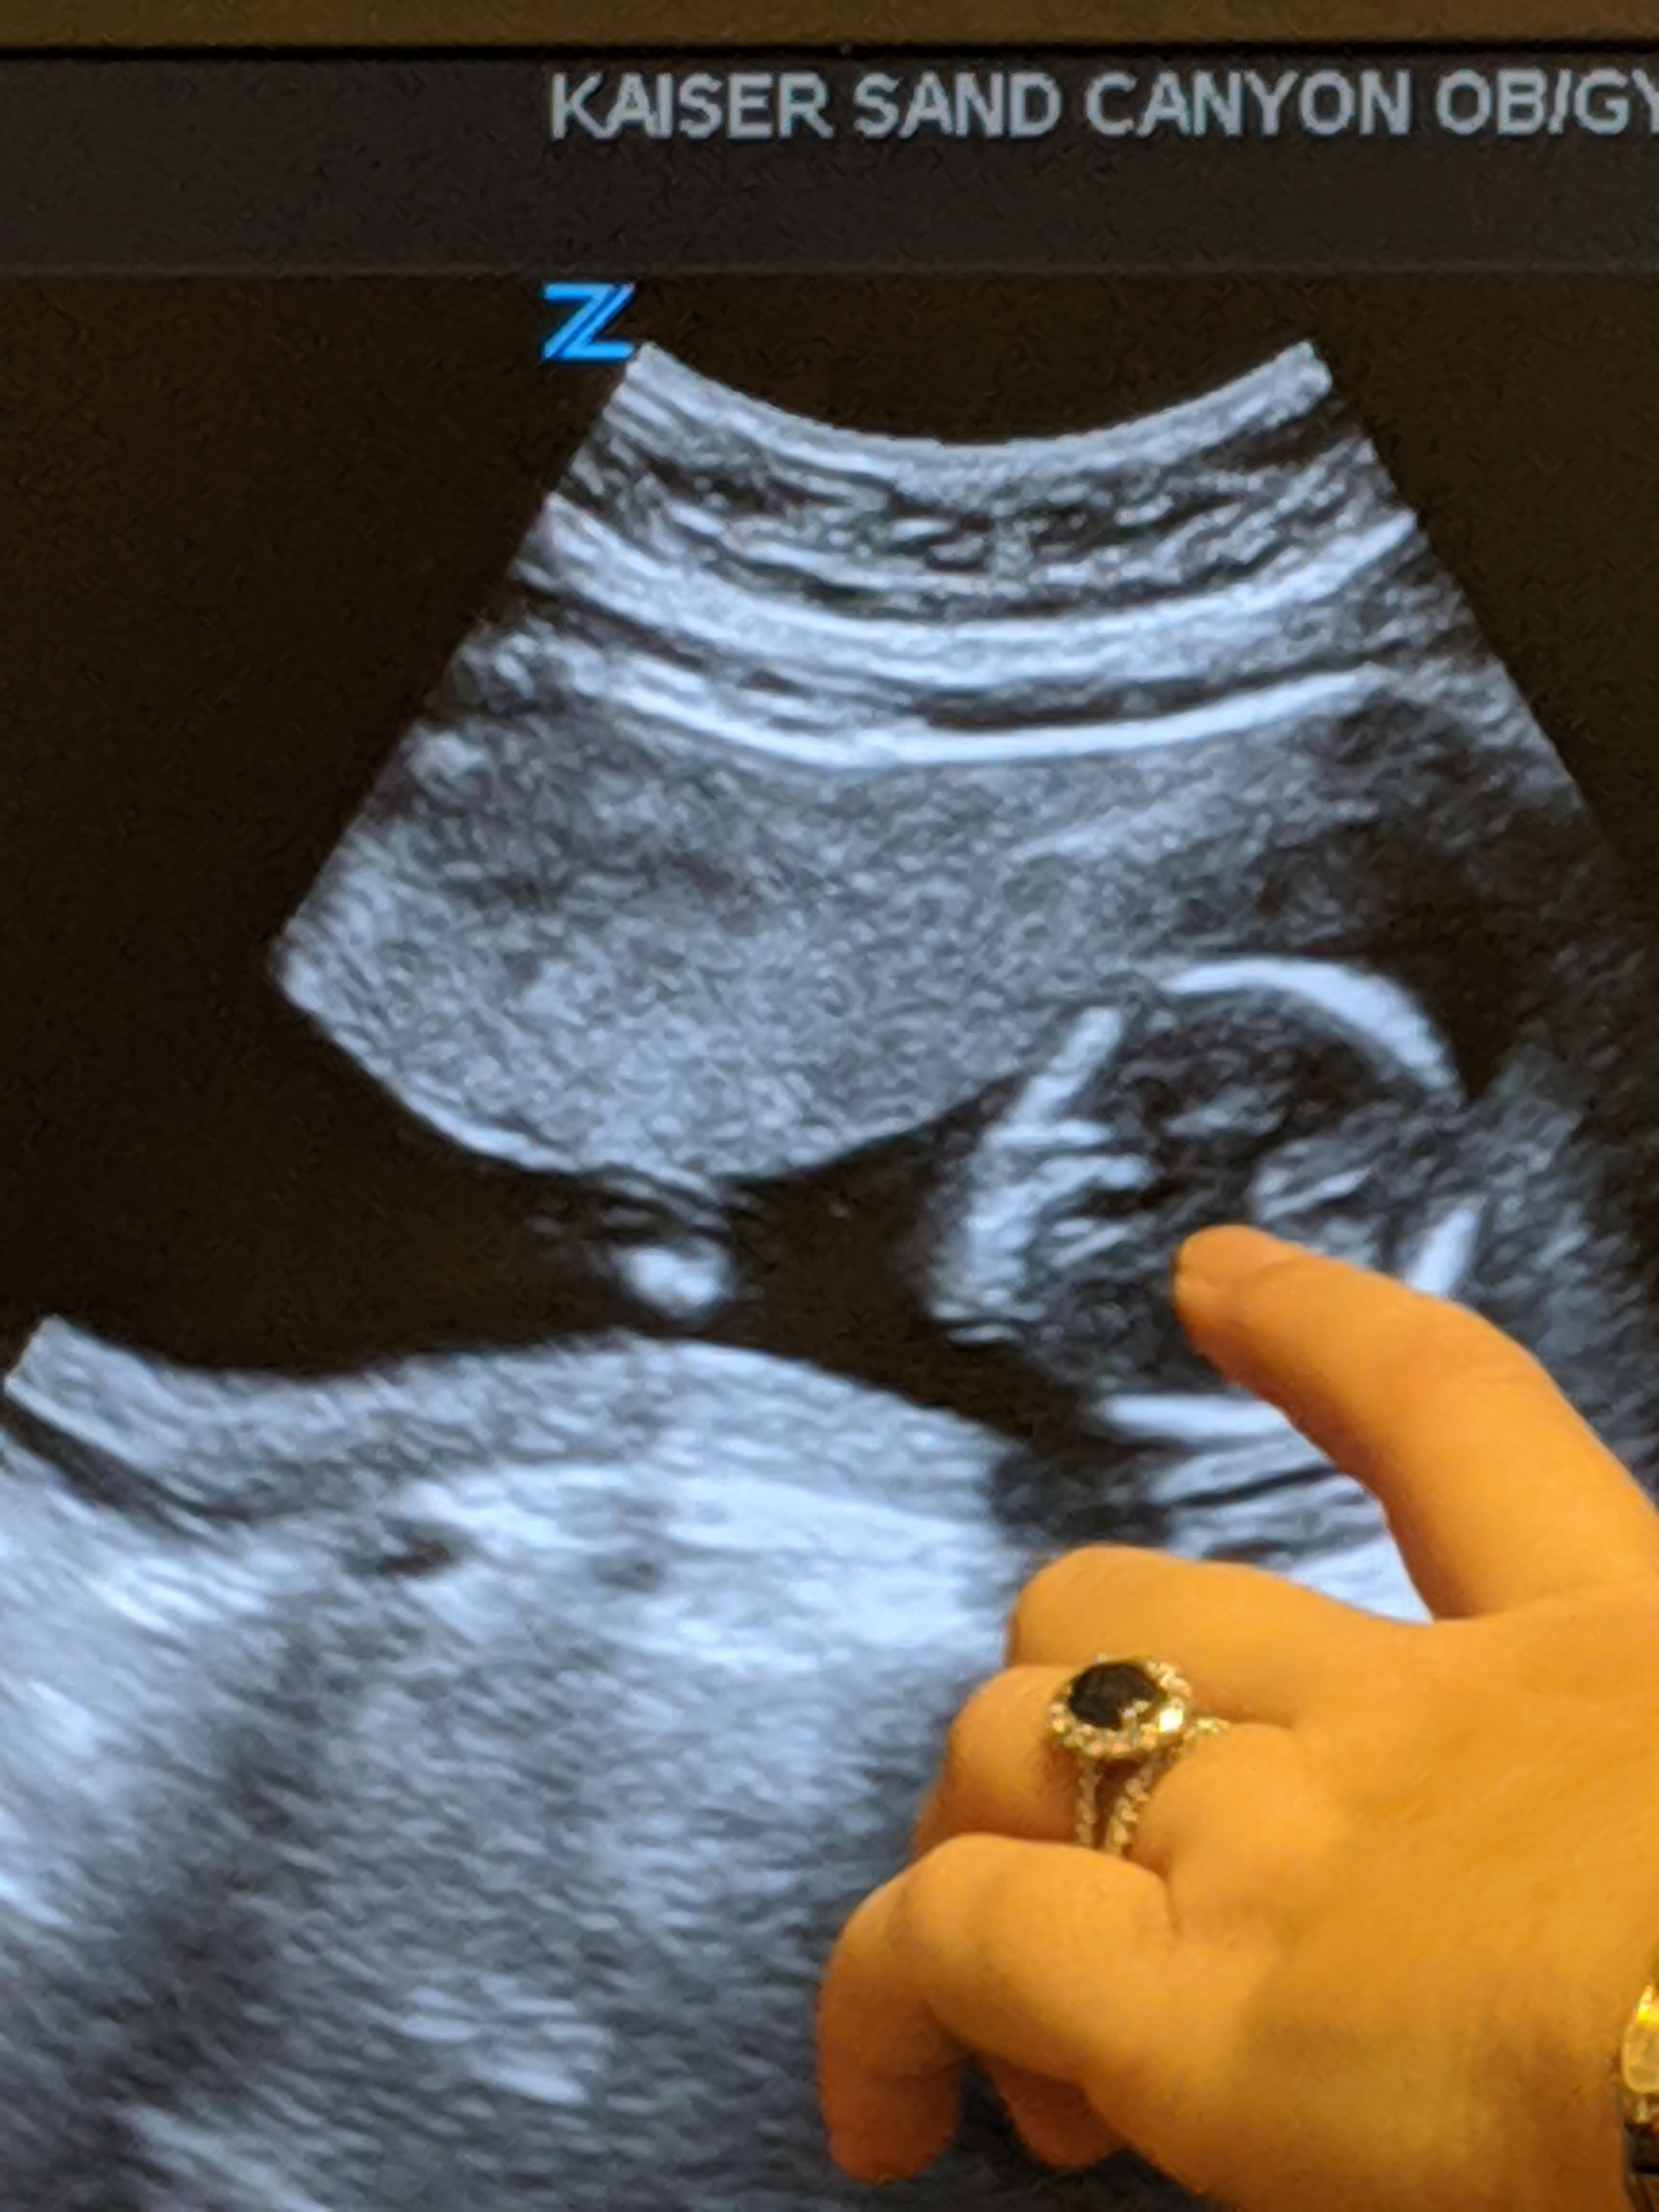
\includegraphics[width=0.5\textwidth]{IMG_20191108_073729.jpg}
\end{figure}
\end{frame}

\begin{frame}{Thank you}
\begin{figure}
\centering
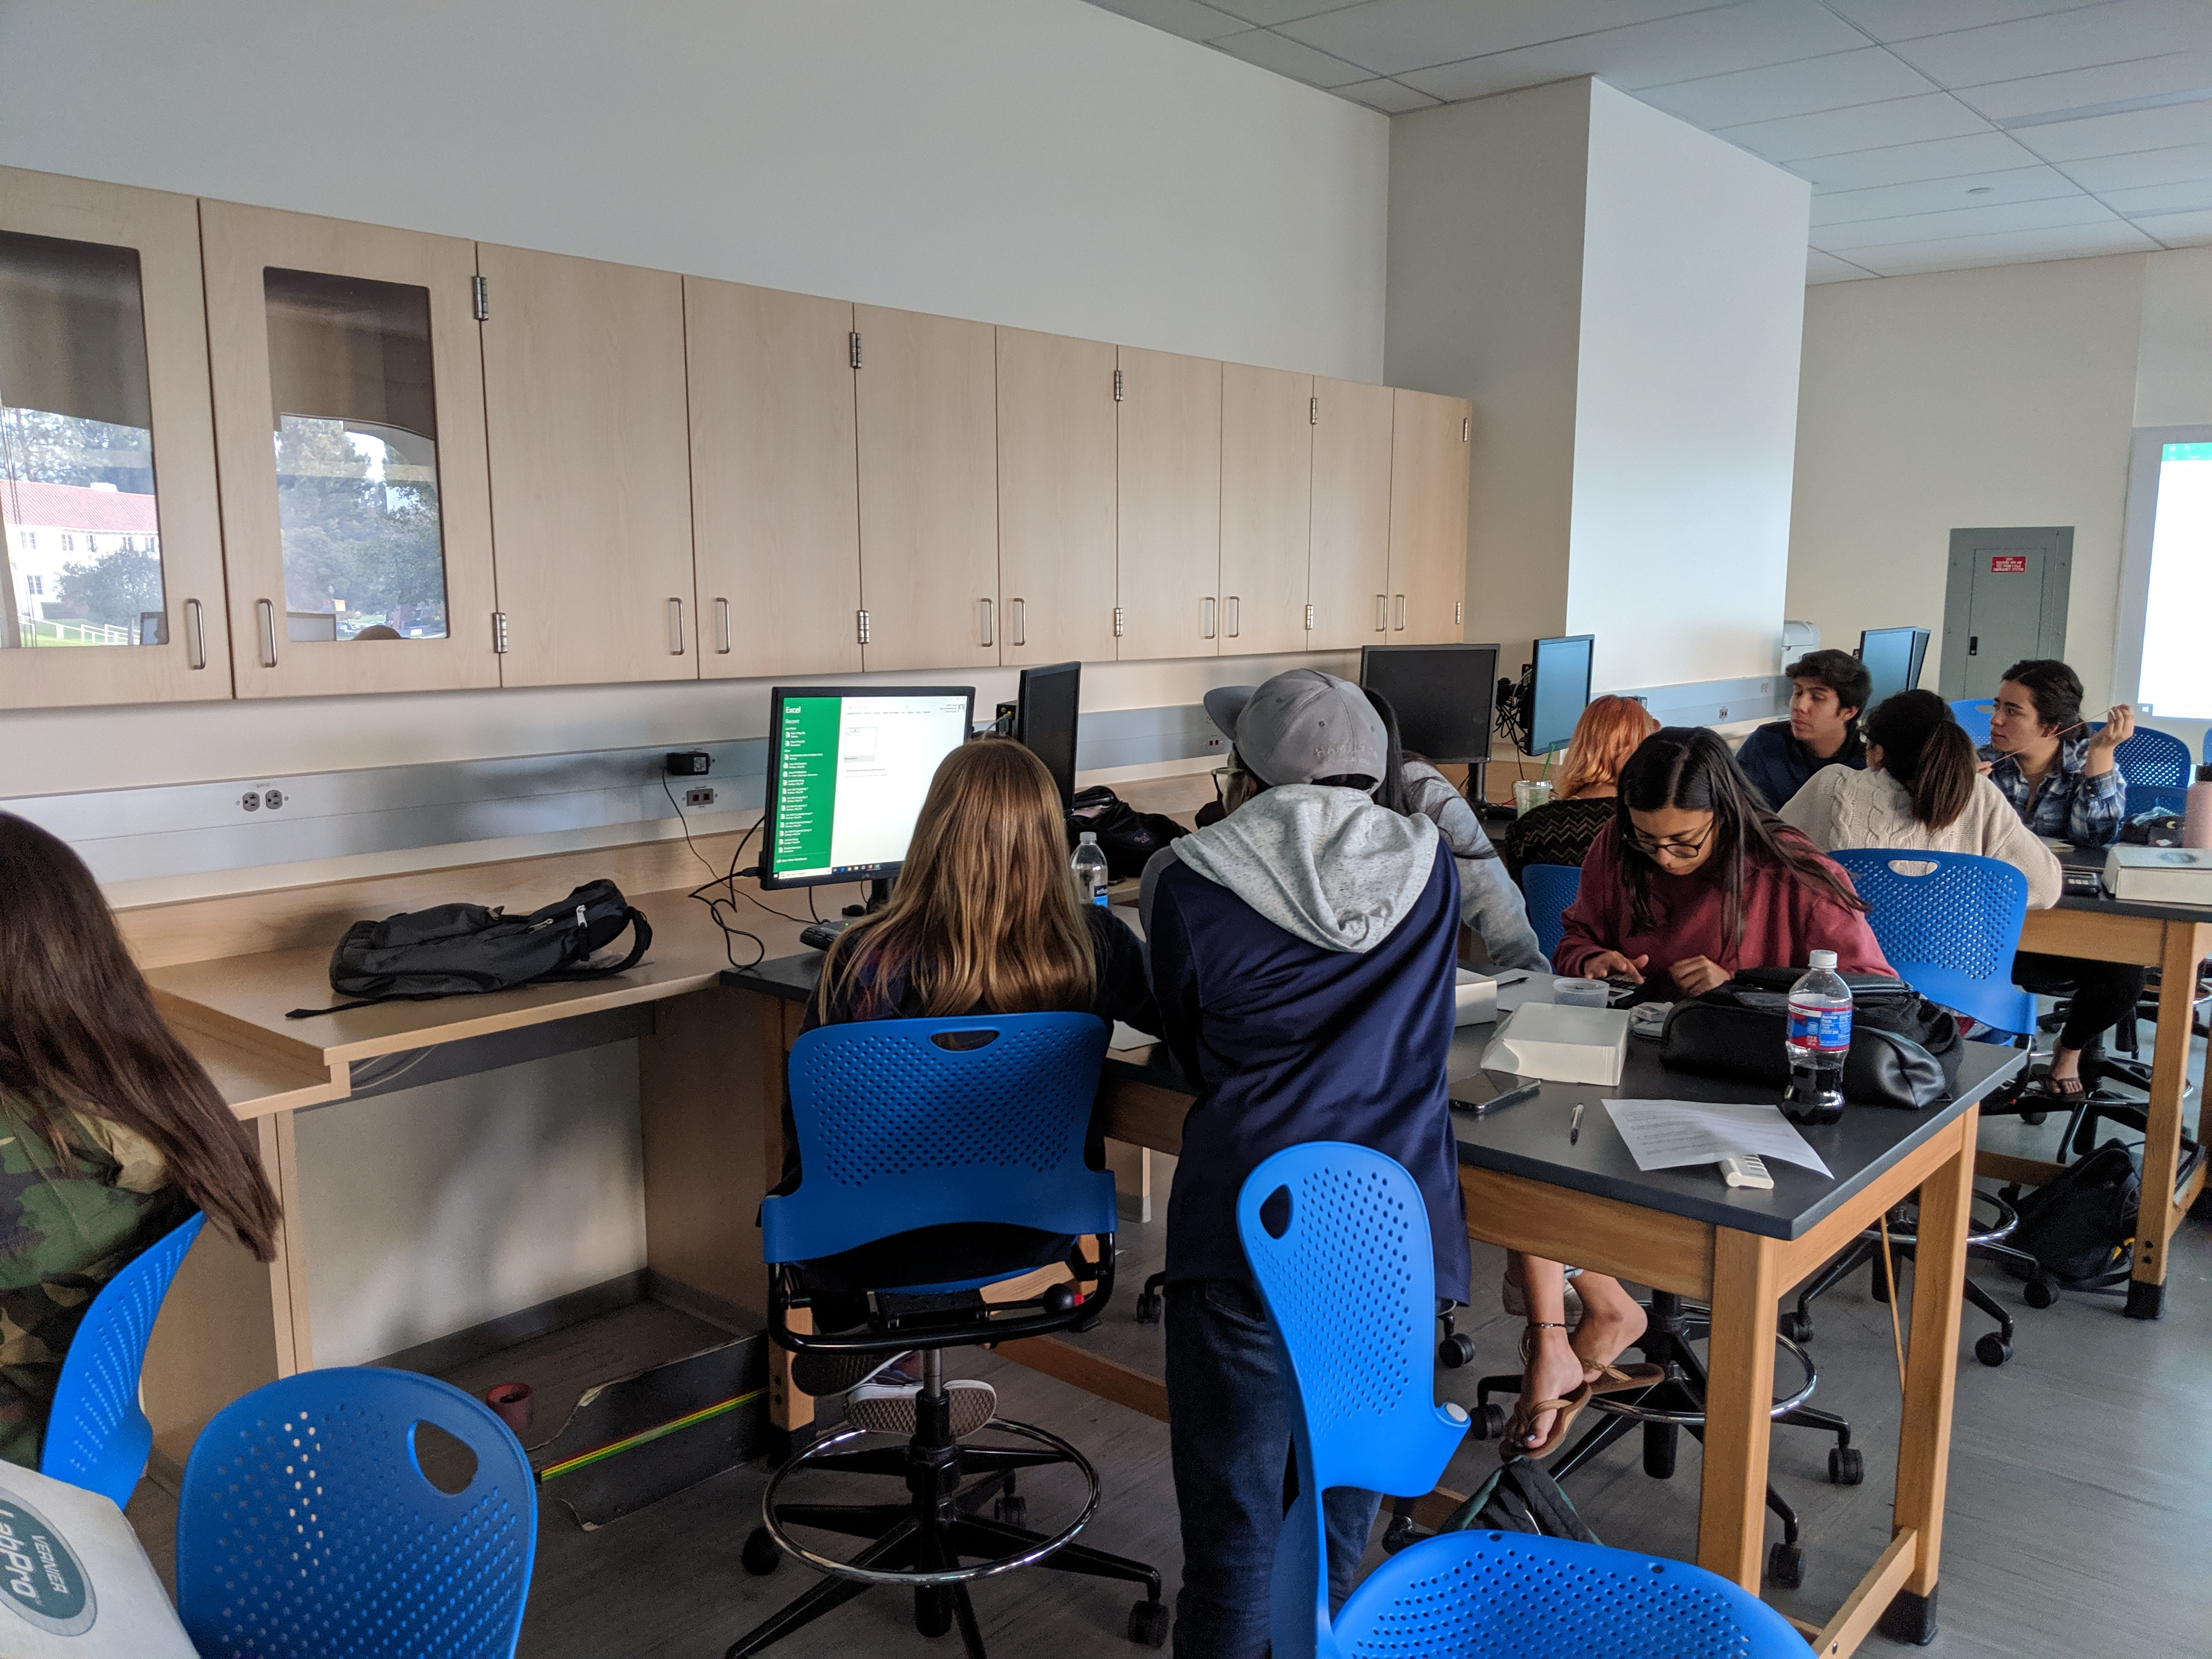
\includegraphics[width=0.75\textwidth]{IMG_20191113_153819.jpg}
\end{figure}
\end{frame}

\begin{frame}{Thank you}
\begin{figure}
\centering
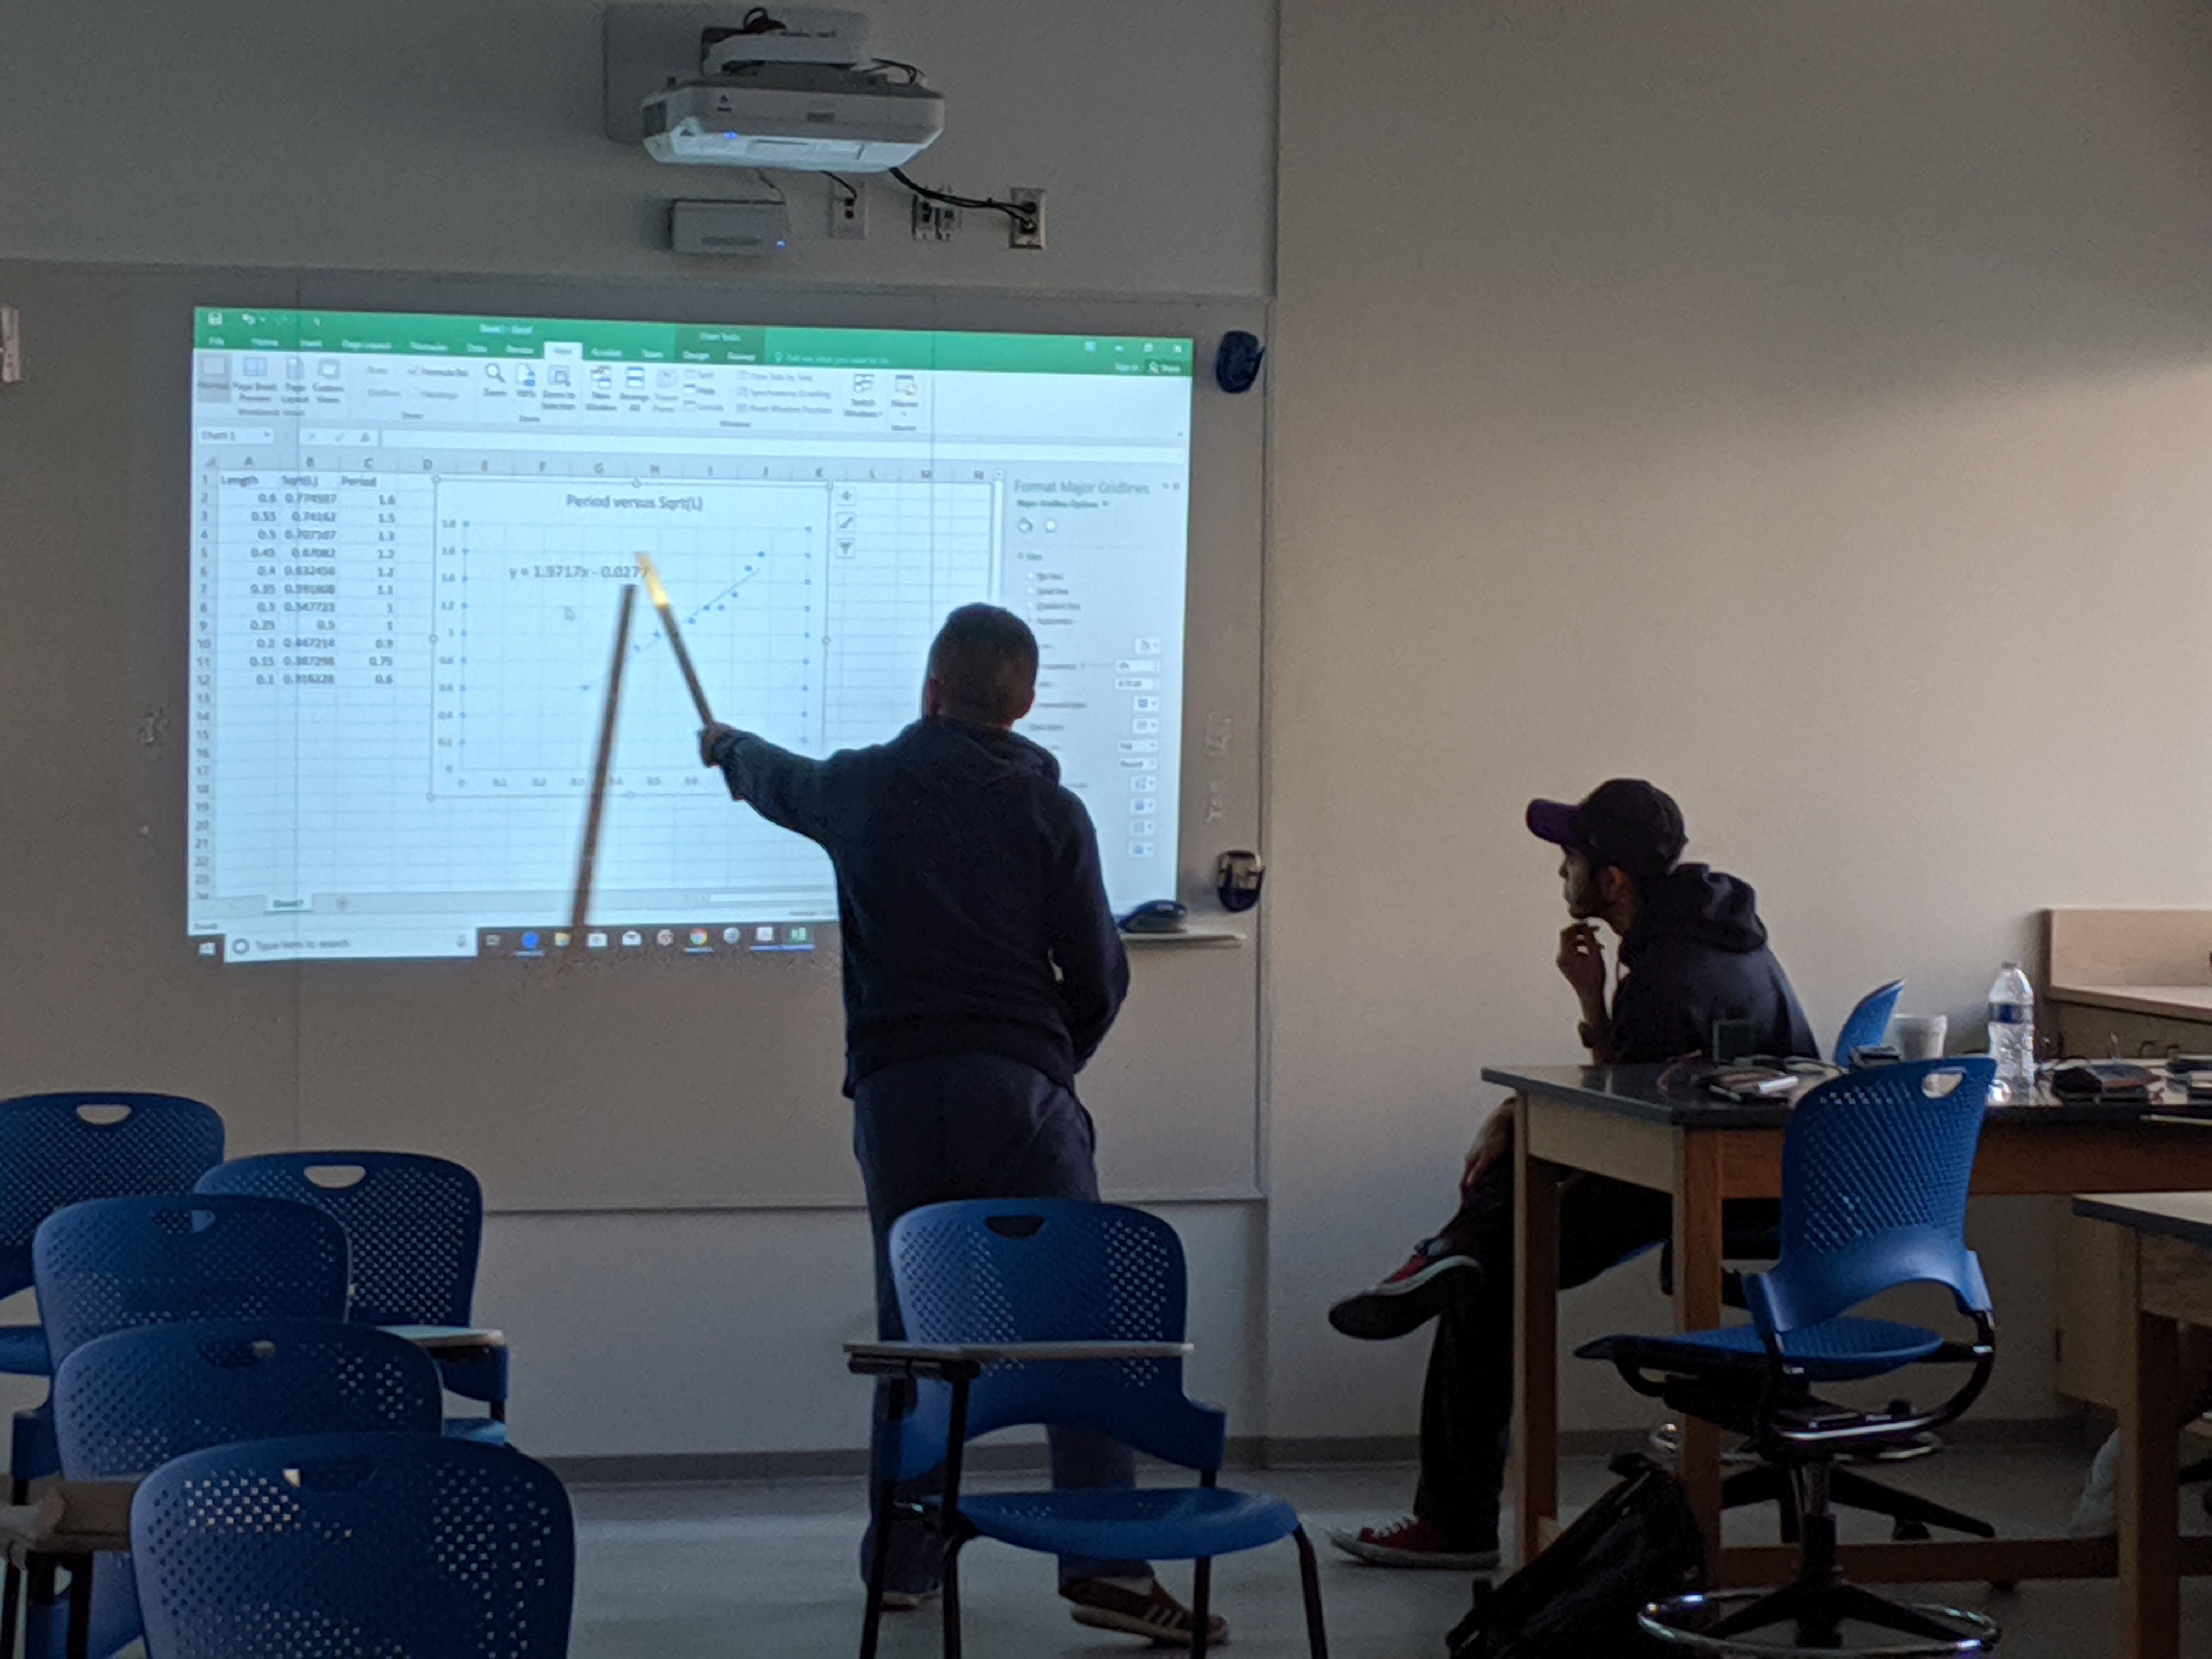
\includegraphics[width=0.75\textwidth]{IMG_20191113_153800.jpg}
\end{figure}
\end{frame}

\begin{frame}{Thank you}
\begin{figure}
\centering
\includegraphics[width=0.5\textwidth]{IMG_20191026_093138.jpg}
\end{figure}
\end{frame}

\section{Thank you.}

\end{document}
